% !TeX spellcheck = en_US

% We need layers to draw the block diagram
\usetikzlibrary{calc,positioning}
\usetikzlibrary{arrows.meta}

% Define a few styles and constants
\tikzstyle{entry}=[draw, fill=green!20, minimum height=2.5em]
\tikzstyle{ann} = [above, text width=5em]
\tikzstyle{item} = [entry, text width=7em, shading = axis,rectangle, left color=blue!10!white, right color=blue!30!white,shading angle=135, anchor=north,
minimum height=2em, rounded corners, align=center]
%\def\blockdist{2.3}
%\def\edgedist{2.5}

\begin{figure}
	\centering
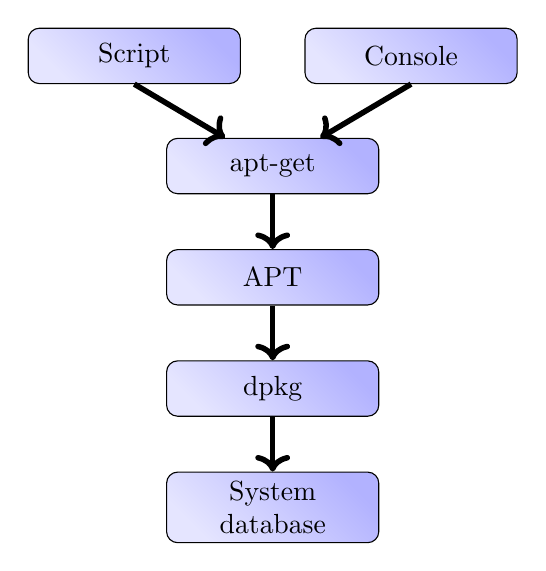
\begin{tikzpicture}
\node (aptget) [item] {apt-get};
\node (console) [yshift=+5em, xshift=+5em] at ( aptget) [item] {Console};
\node (script) [yshift=+5em, xshift=-5em] at ( aptget) [item] {Script};
\node (apt) [yshift=-3em] at ( aptget) [item] {APT};
\node (dpkg) [yshift=-3em] at (apt) [item] {dpkg};
\node (system) [yshift=-3em] at (dpkg) [item] {System database};

\draw [->,scale=1,line width=2pt] (console.south) -- (aptget);
\draw [->,scale=2,line width=2pt] (script.south) -- (aptget);
\draw [->,scale=2,line width=2pt] (aptget) -- (apt);
\draw [->,scale=2,line width=2pt] (apt) -- (dpkg);
\draw [->,scale=2,line width=2pt] (dpkg) -- (system);
\end{tikzpicture} 
\caption{Package management} 	\label{fig:packages}
\end{figure}